\section{风险概述}
\subsection{风险分类}

风险分为一下几类:
\begin{figure}[H]
	\centering
	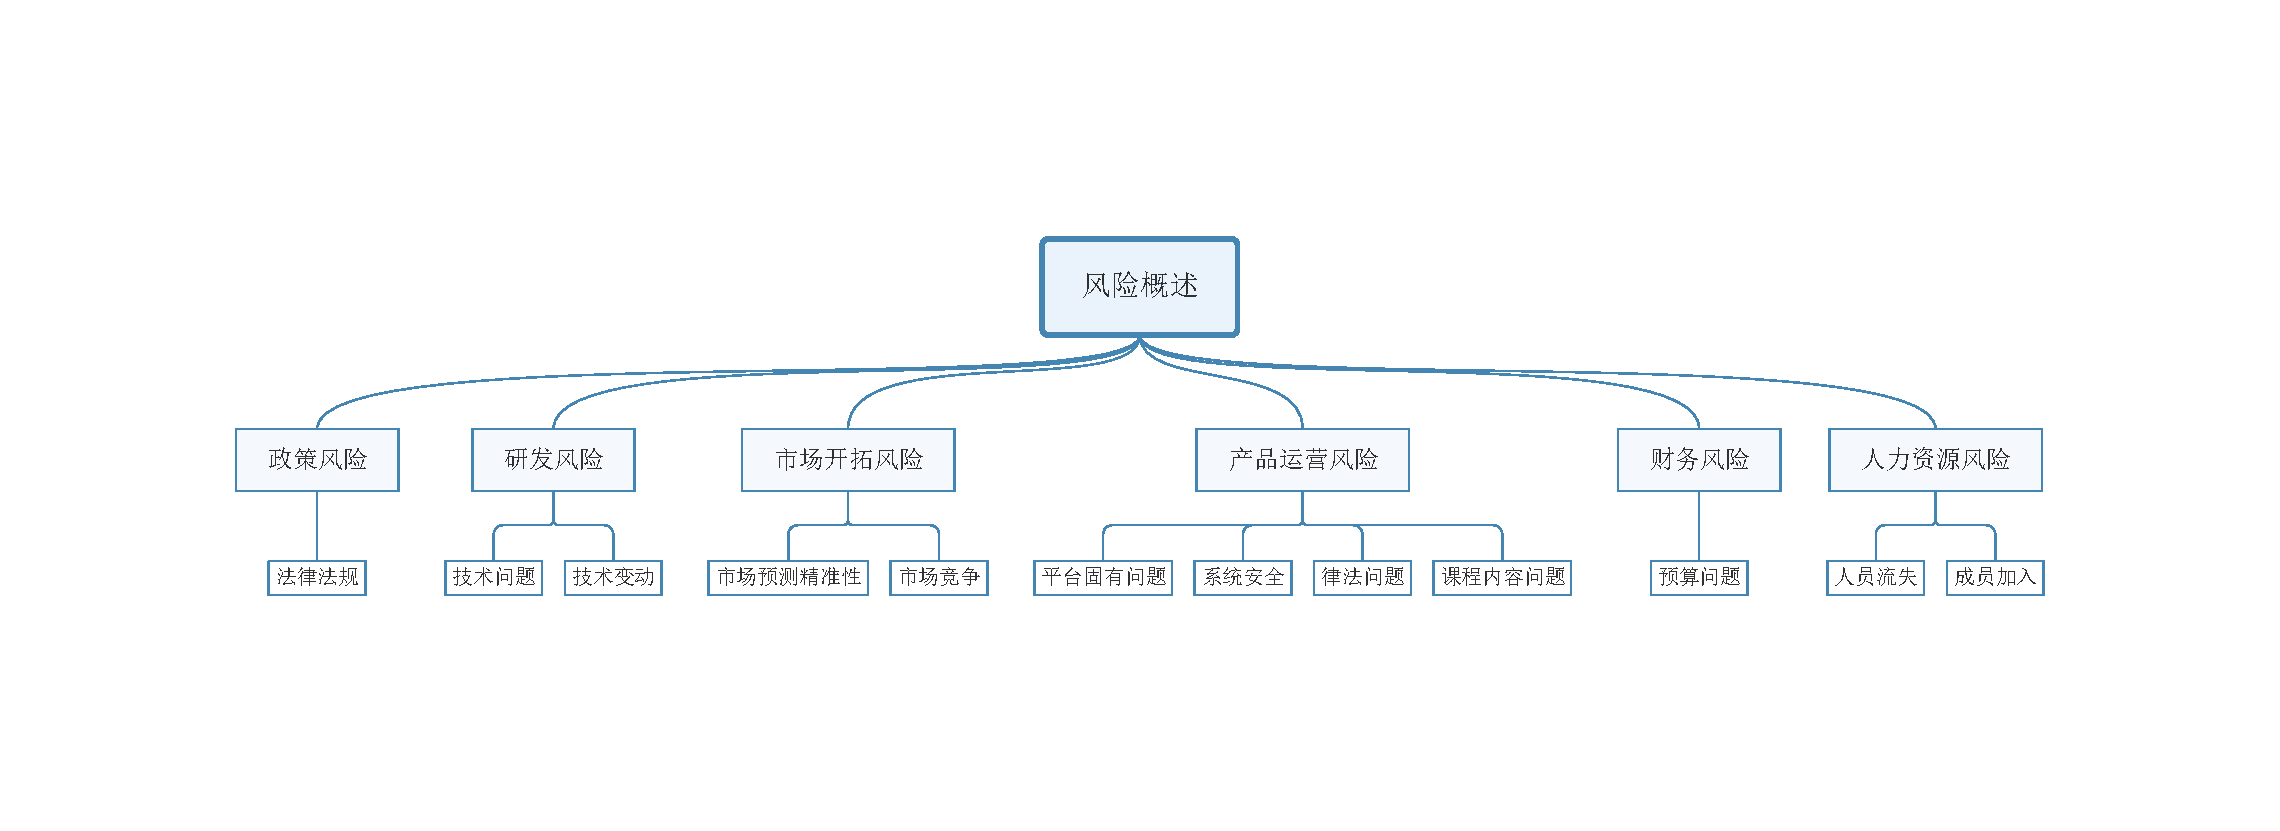
\includegraphics[width=0.9\columnwidth]{figures/risk_summary}
	%  \setlength{\abovecaptionskip}{0pt}
	%  \setlength{\belowcaptionskip}{-20pt}
	\caption{风险概述}
	\label{fg:risk_summary}
\end{figure}

\subsection{风险控制}

公司的创立与发展总是风险与机遇共存,想要发展成一个行业的领导者必定会面临各个方面带来的各种压力。所谓“知己知彼,百战不殆”,提前对可能遇到的风险做一个较为完全的预估是公司长久发展的基础。在充分考虑了政策、市场、产品运营、财务等各方面因素之后,本公司对发展中可能遇到的风险做了比较全面地评估,并提出了统一的风险控制模型以减少不必要的风险及可能带来的损失。

\begin{figure}[H]
	\centering
	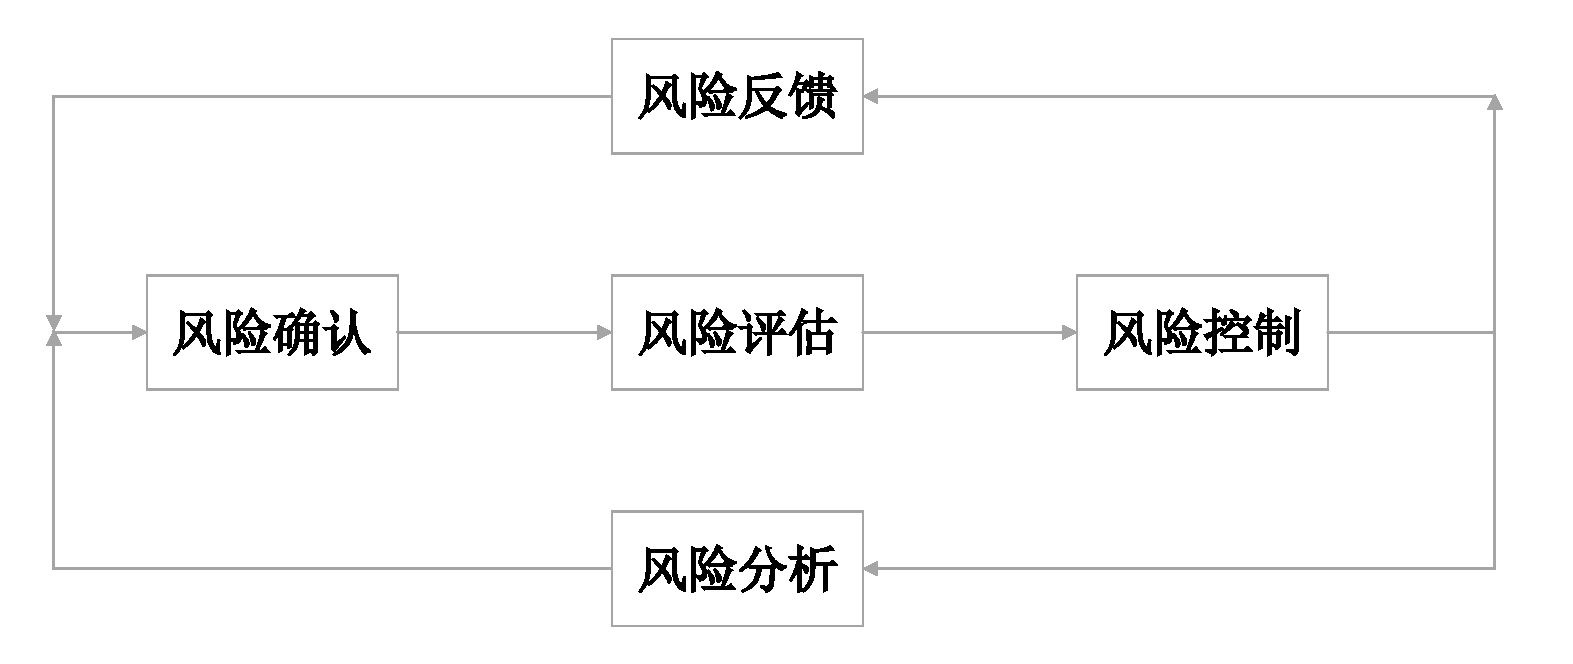
\includegraphics[width=0.9\columnwidth]{figures/rist_control}
	%  \setlength{\abovecaptionskip}{0pt}
	%  \setlength{\belowcaptionskip}{-20pt}
	\caption{风险控制}
	\label{fg:rist_control}
\end{figure}


\subsection{风险概览}
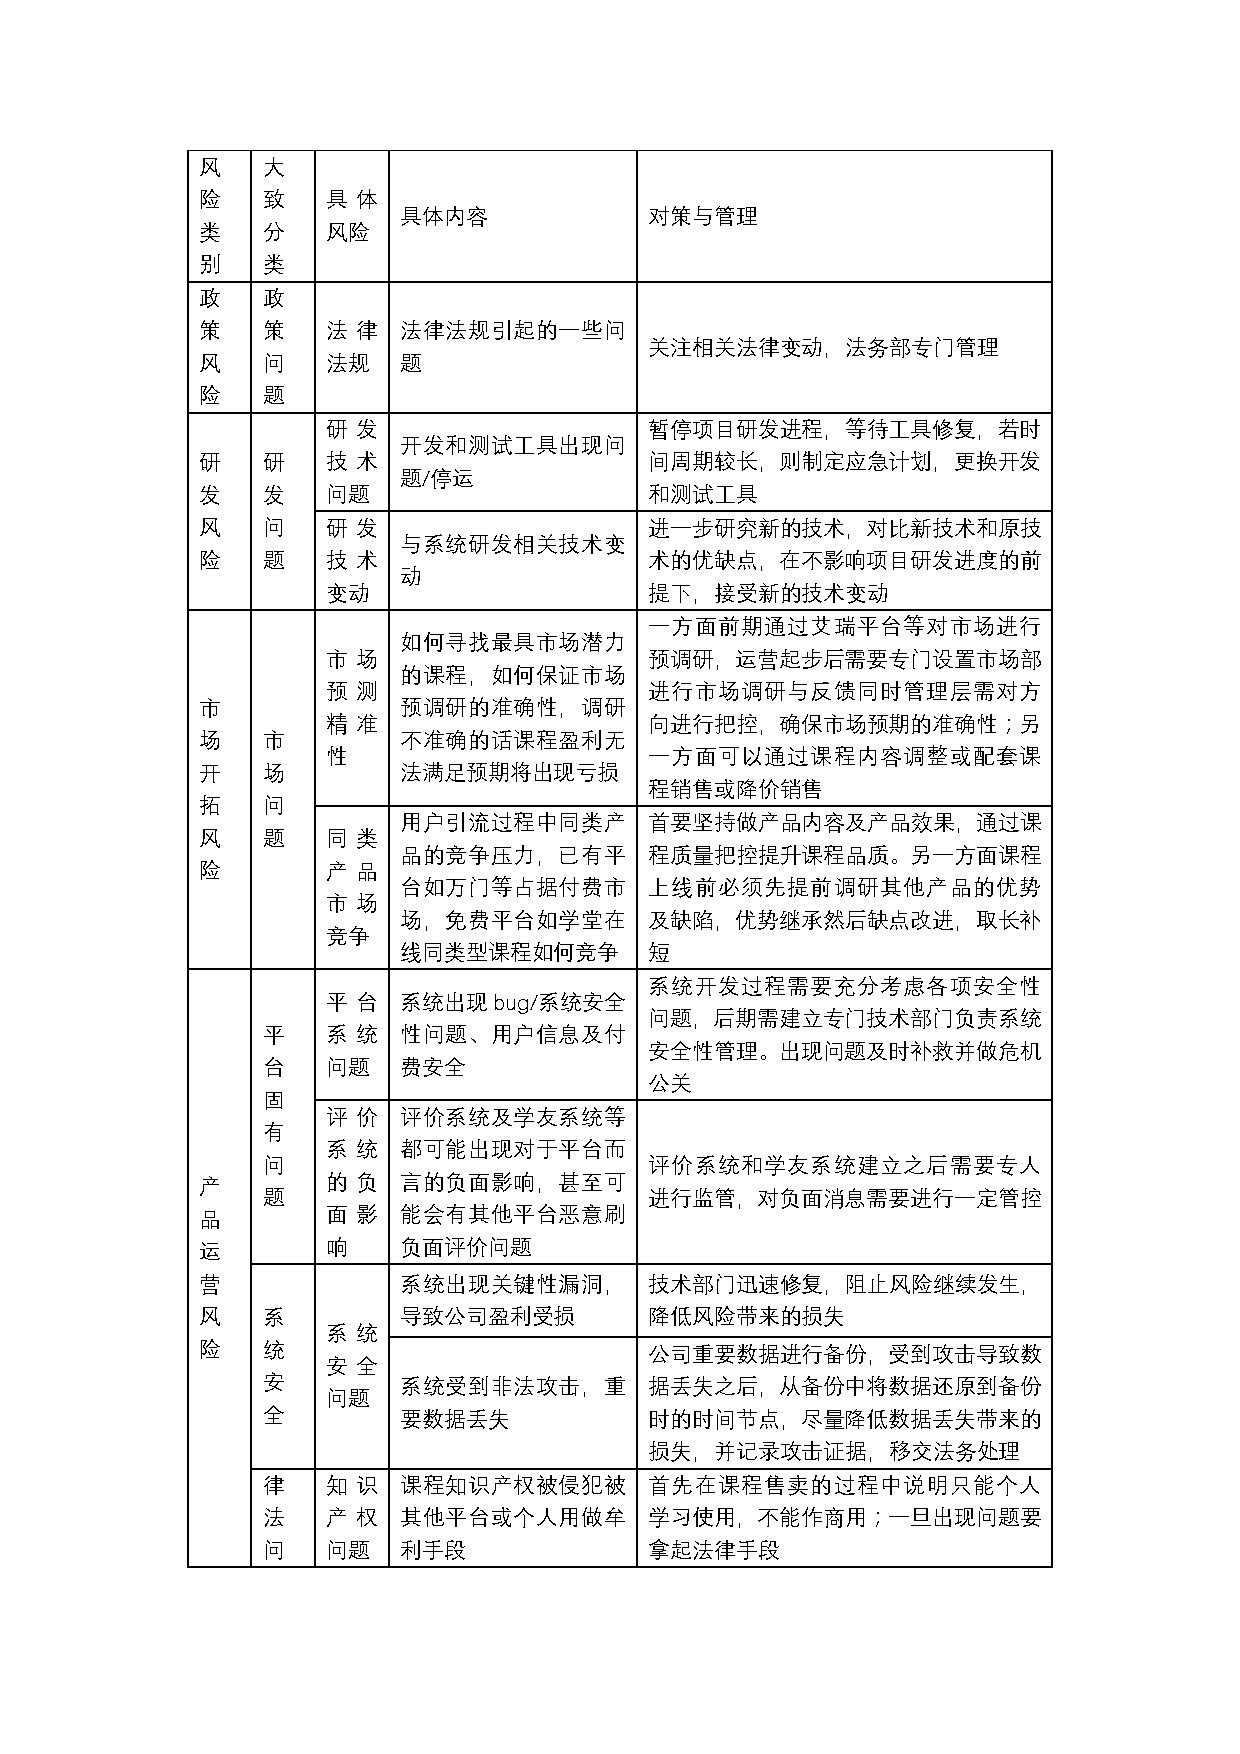
\includepdf{data/fxgs1.pdf}
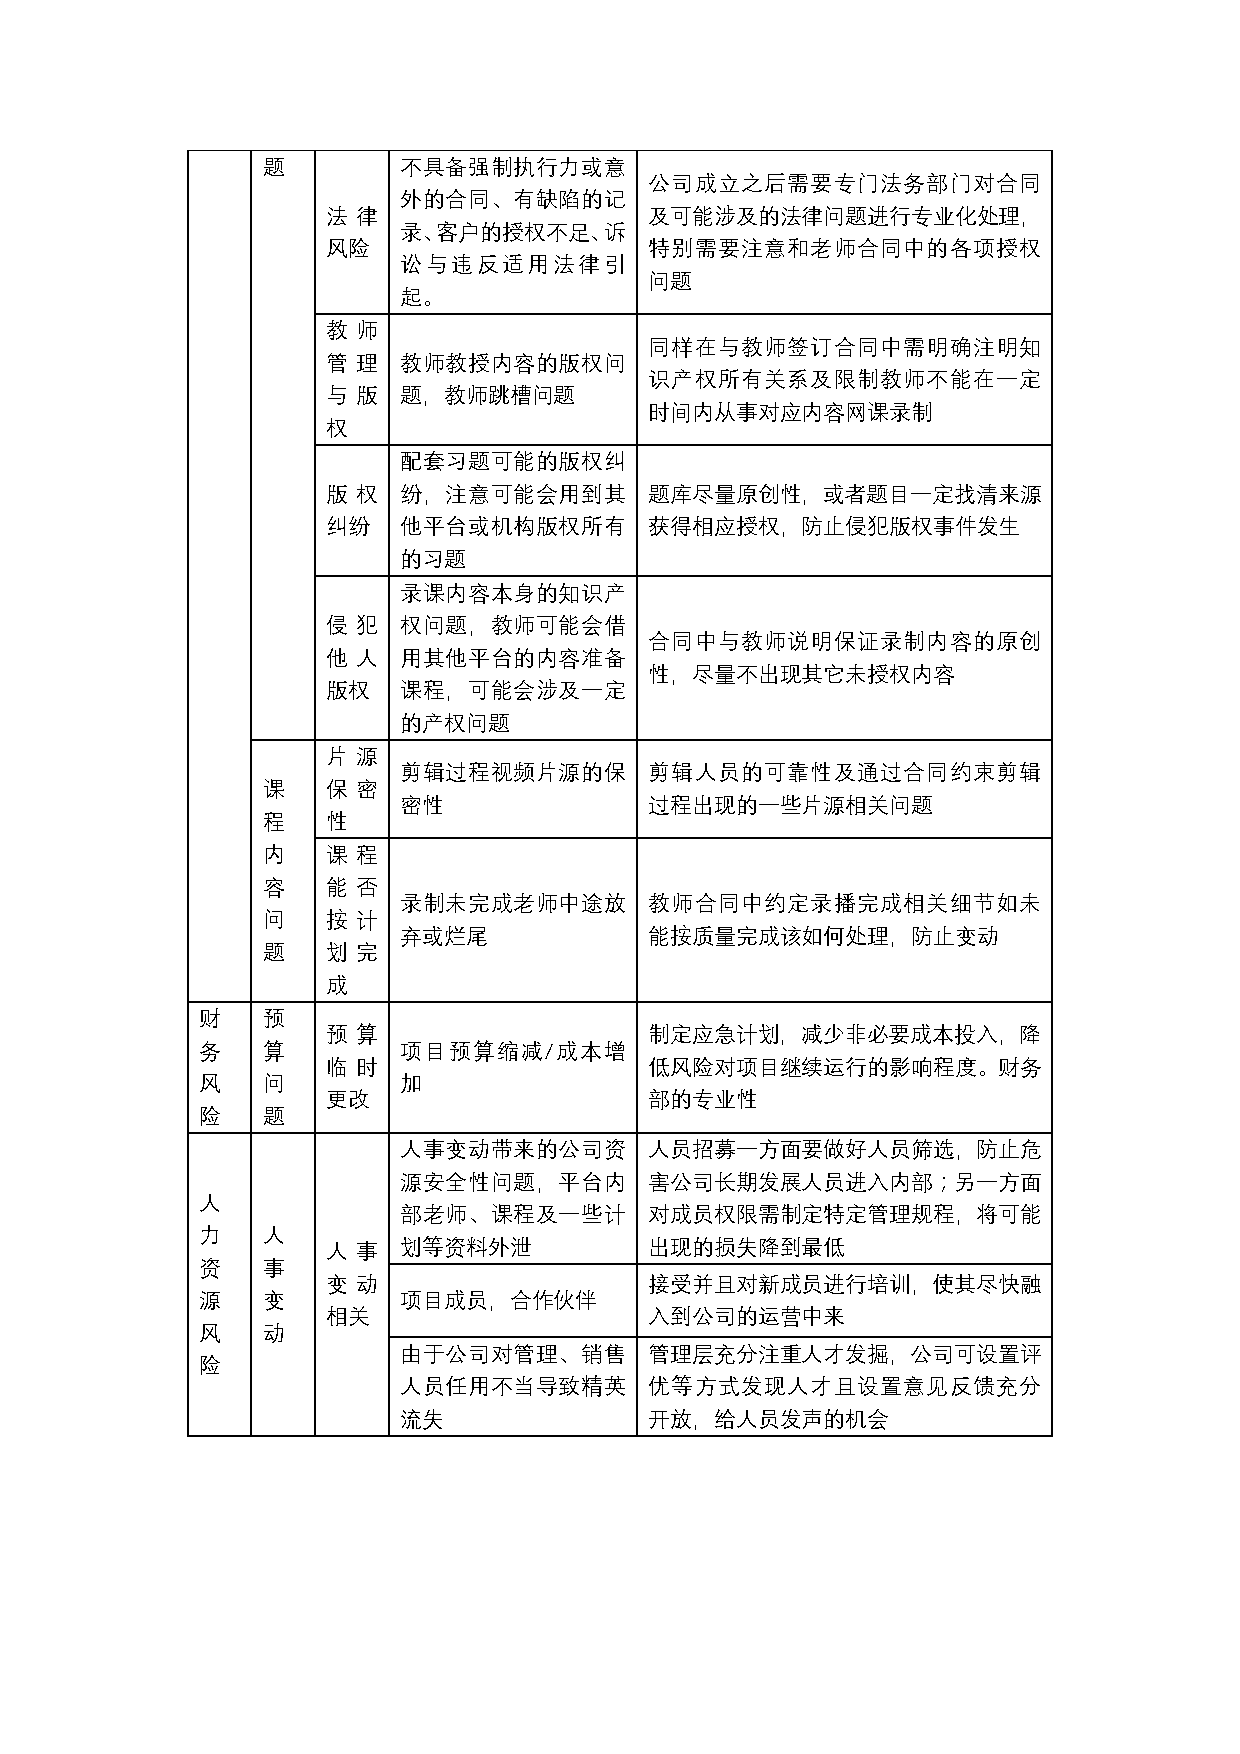
\includepdf{data/fxgs2.pdf}